\documentclass[xcolor={usenames,dvipsnames}, aspectratio=169, 12pt]{beamer}
\usetheme{tum}

\usepackage[utf8]{inputenc}
\usepackage[T1]{fontenc}
\usepackage[english]{babel}
\usepackage{amsmath}
\usepackage{dsfont}
\usepackage{wasysym}
\usepackage{calc}
\usepackage{xcolor}
\usepackage{tikz}
\usetikzlibrary{positioning, calc, arrows.meta}
\usepackage{listings}
\usepackage{stmaryrd}
\usepackage{svg}
\usepackage{graphicx}

\lstset{
	numbers=left,
	numberstyle=\tiny\color{gray},
	stepnumber=1,
	numbersep=5pt,
	showspaces=false,
	showstringspaces=false,
	showtabs=false,
	frame=single,
	rulecolor=\color{black},
	tabsize=4,
	captionpos=b,
	breaklines=true,
	breakatwhitespace=false,
	language=Java,
	commentstyle=\itshape\color{RubineRed},
	stringstyle=\color{BrickRed},
	keywordstyle=\bfseries\color{Purple},
	keywordstyle=[2]{\color{MidnightBlue}},
	keywordstyle=[3]{\color{RoyalPurple}},
	escapechar=ß,
	xleftmargin=8pt,
	xrightmargin=3pt,
	basicstyle=\scriptsize\ttfamily,
	morekeywords={function, in, not},
	morecomment=[n][\color{RoyalBlue}]{<}{>}
}

% META
% =========================================================
\title[Program Optimization]{Constant Propagation}
%\subtitle{}
\author[B.Pöttinger]{Bernhard Pöttinger}
\date{March 7, 2019}
% Drop the following 2 lines if your title page is too full
\institute{Technische Universität München}
%\semester{SS 2017}

% =========================================================

\begin{document}

\frame[plain]{\titlepage}

%%%%%%%%%%%%%%%%%%%%%%%%%%%%%%%%%%%%%%%%%%%%%%%%%%%%%%%%%%%%%%%%%%%%%%%%%%%%%%
\begin{frame}{Constant Propagation}
	The Analysis:
	\begin{enumerate}
		\item The domain is $\mathbb D = (\texttt{Var} \to \mathbb{Z}^{\top})_{\bot}$ (same as in lecture).
		\item The analysis only considers signed integers of a size of 32 bits.
		\item The analysis is intraprocedural, i.e. it does not allow function or procedure calls.
		\item Edge effects for assignments, nops and guards are implemented analogously to lecture.
		\item Our $\Psi$-edges are evaluated as parallel assignments.
	\end{enumerate}
\end{frame}

%%%%%%%%%%%%%%%%%%%%%%%%%%%%%%%%%%%%%%%%%%%%%%%%%%%%%%%%%%%%%%%%%%%%%%%%%%%%%%
\begin{frame}{Constant Propagation}
	Abstract Interpretation:
	\begin{enumerate}
		\item Extended version from the lecture with evaluation and substitution of subexpressions.
		\item Algebraic optimizations for binary expressions involving additive and multiplicative neutral elements.
		\item Traversal over syntax-tree substitutes subtrees with known value.
		\item Function calls again are not allowed.
		\item Divison by zero is kept to not alter side-effects.
	\end{enumerate}
\end{frame}

%%%%%%%%%%%%%%%%%%%%%%%%%%%%%%%%%%%%%%%%%%%%%%%%%%%%%%%%%%%%%%%%%%%%%%%%%%%%%%
\begin{frame}{Constant Propagation}
	Transformation:
	\begin{enumerate}
		\item $\Psi$-edges: assignments in parallel.
		\item Otherwise: the same as in the lecture.
	\end{enumerate}
\end{frame}

%%%%%%%%%%%%%%%%%%%%%%%%%%%%%%%%%%%%%%%%%%%%%%%%%%%%%%%%%%%%%%%%%%%%%%%%%%%%%%
\begin{frame}{Constant Propagation}
	Example: Partial Substitution and Algebraic Optimization

	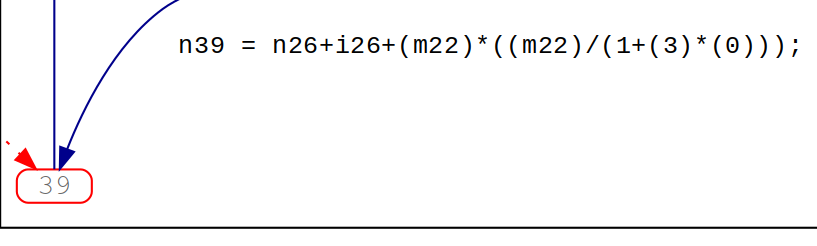
\includegraphics[width=\linewidth]{images/constfolding/example1a.png}

	\texttt{m22} is constant and algebraic simplifications can be applied.
\end{frame}

%%%%%%%%%%%%%%%%%%%%%%%%%%%%%%%%%%%%%%%%%%%%%%%%%%%%%%%%%%%%%%%%%%%%%%%%%%%%%%
\begin{frame}{Constant Propagation}
	Example: Partial Substitution and Algebraic Optimization

	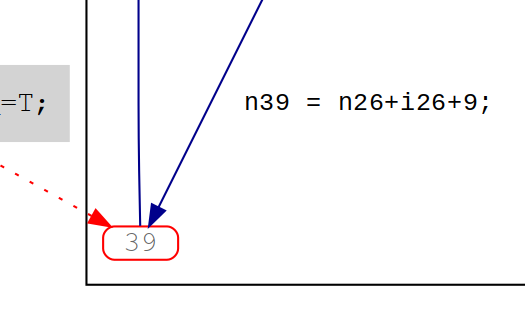
\includegraphics[width=\linewidth]{images/constfolding/example1b.png}

	\texttt{m22*(m22/1+3*0) = m22*m22 = 3*3 = 9}
\end{frame}

%%%%%%%%%%%%%%%%%%%%%%%%%%%%%%%%%%%%%%%%%%%%%%%%%%%%%%%%%%%%%%%%%%%%%%%%%%%%%%
\begin{frame}{Constant Propagation}
	Example: $\Psi$-Edges

	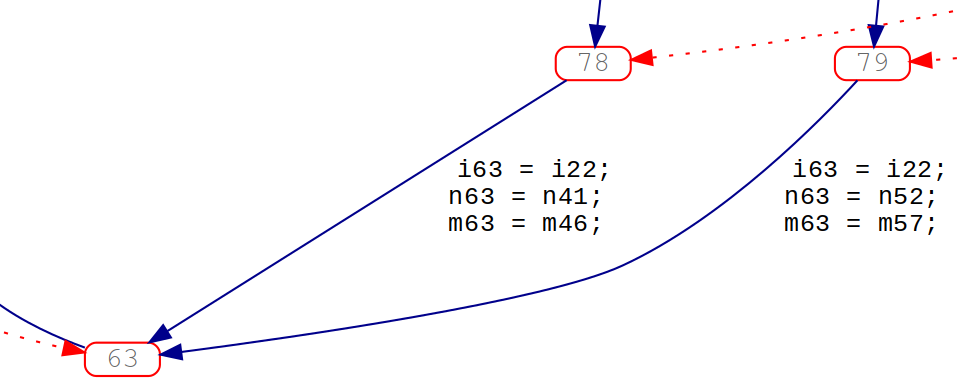
\includegraphics[width=\linewidth]{images/constfolding/example2a.png}

	Redundant assignments of constants on $\Psi$-edge.
\end{frame}

%%%%%%%%%%%%%%%%%%%%%%%%%%%%%%%%%%%%%%%%%%%%%%%%%%%%%%%%%%%%%%%%%%%%%%%%%%%%%%
\begin{frame}{Constant Propagation}
	Example: $\Psi$-Edges

	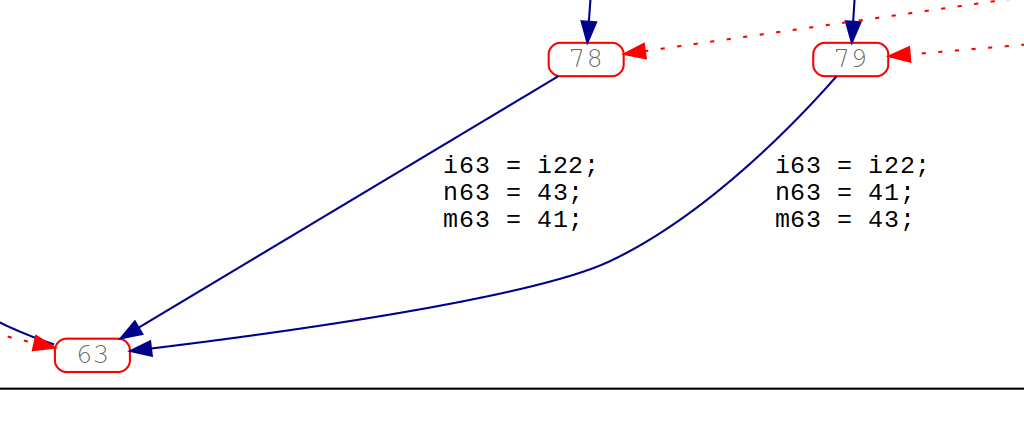
\includegraphics[width=\linewidth]{images/constfolding/example2b.png}

	Evaluate parallel assignments.
\end{frame}

%%%%%%%%%%%%%%%%%%%%%%%%%%%%%%%%%%%%%%%%%%%%%%%%%%%%%%%%%%%%%%%%%%%%%%%%%%%%%%
\begin{frame}{Constant Propagation}
	Example: Removal of Dead Code

	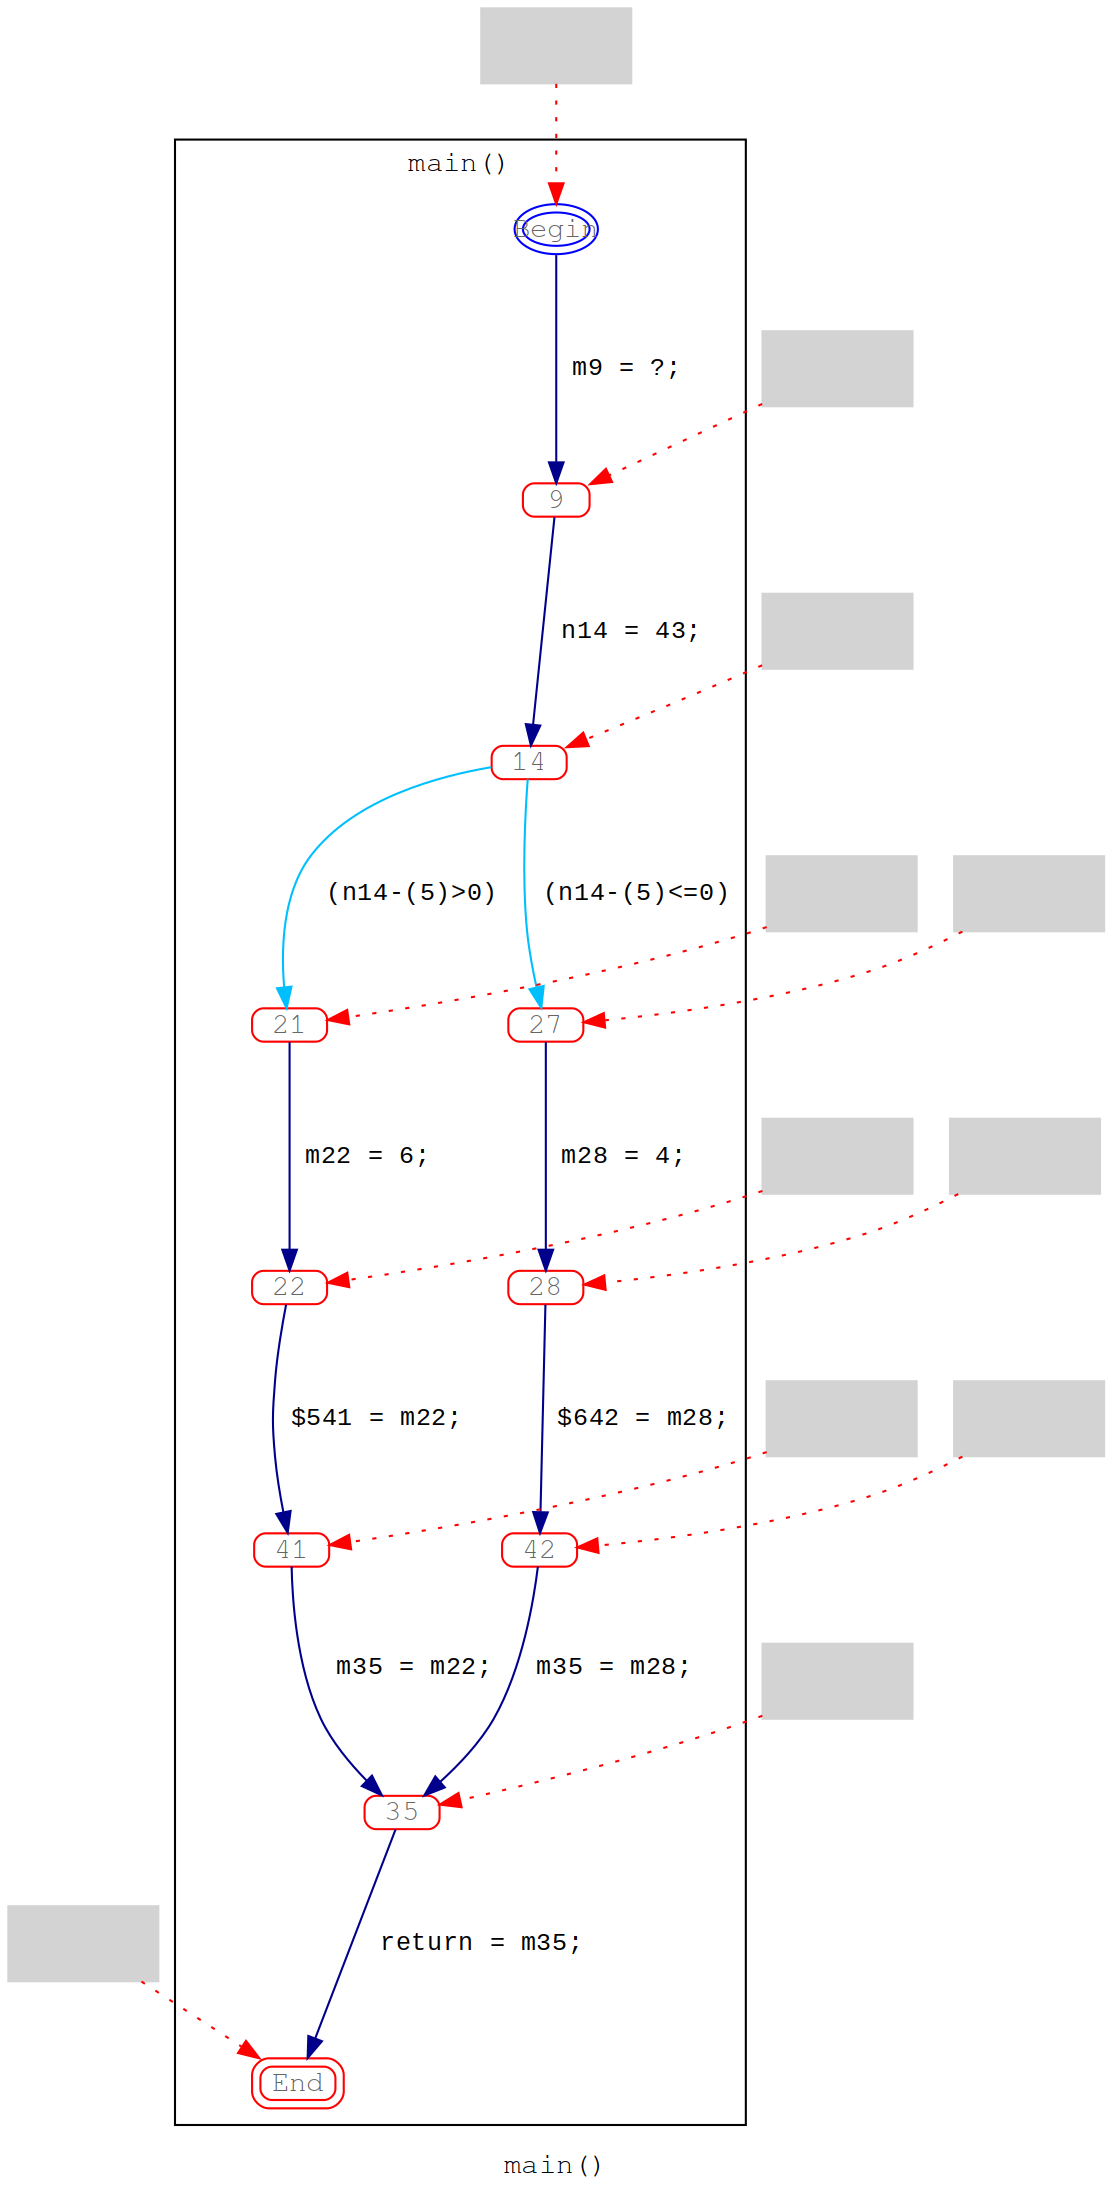
\includegraphics[height=7cm]{images/constfolding/example3a.png}
	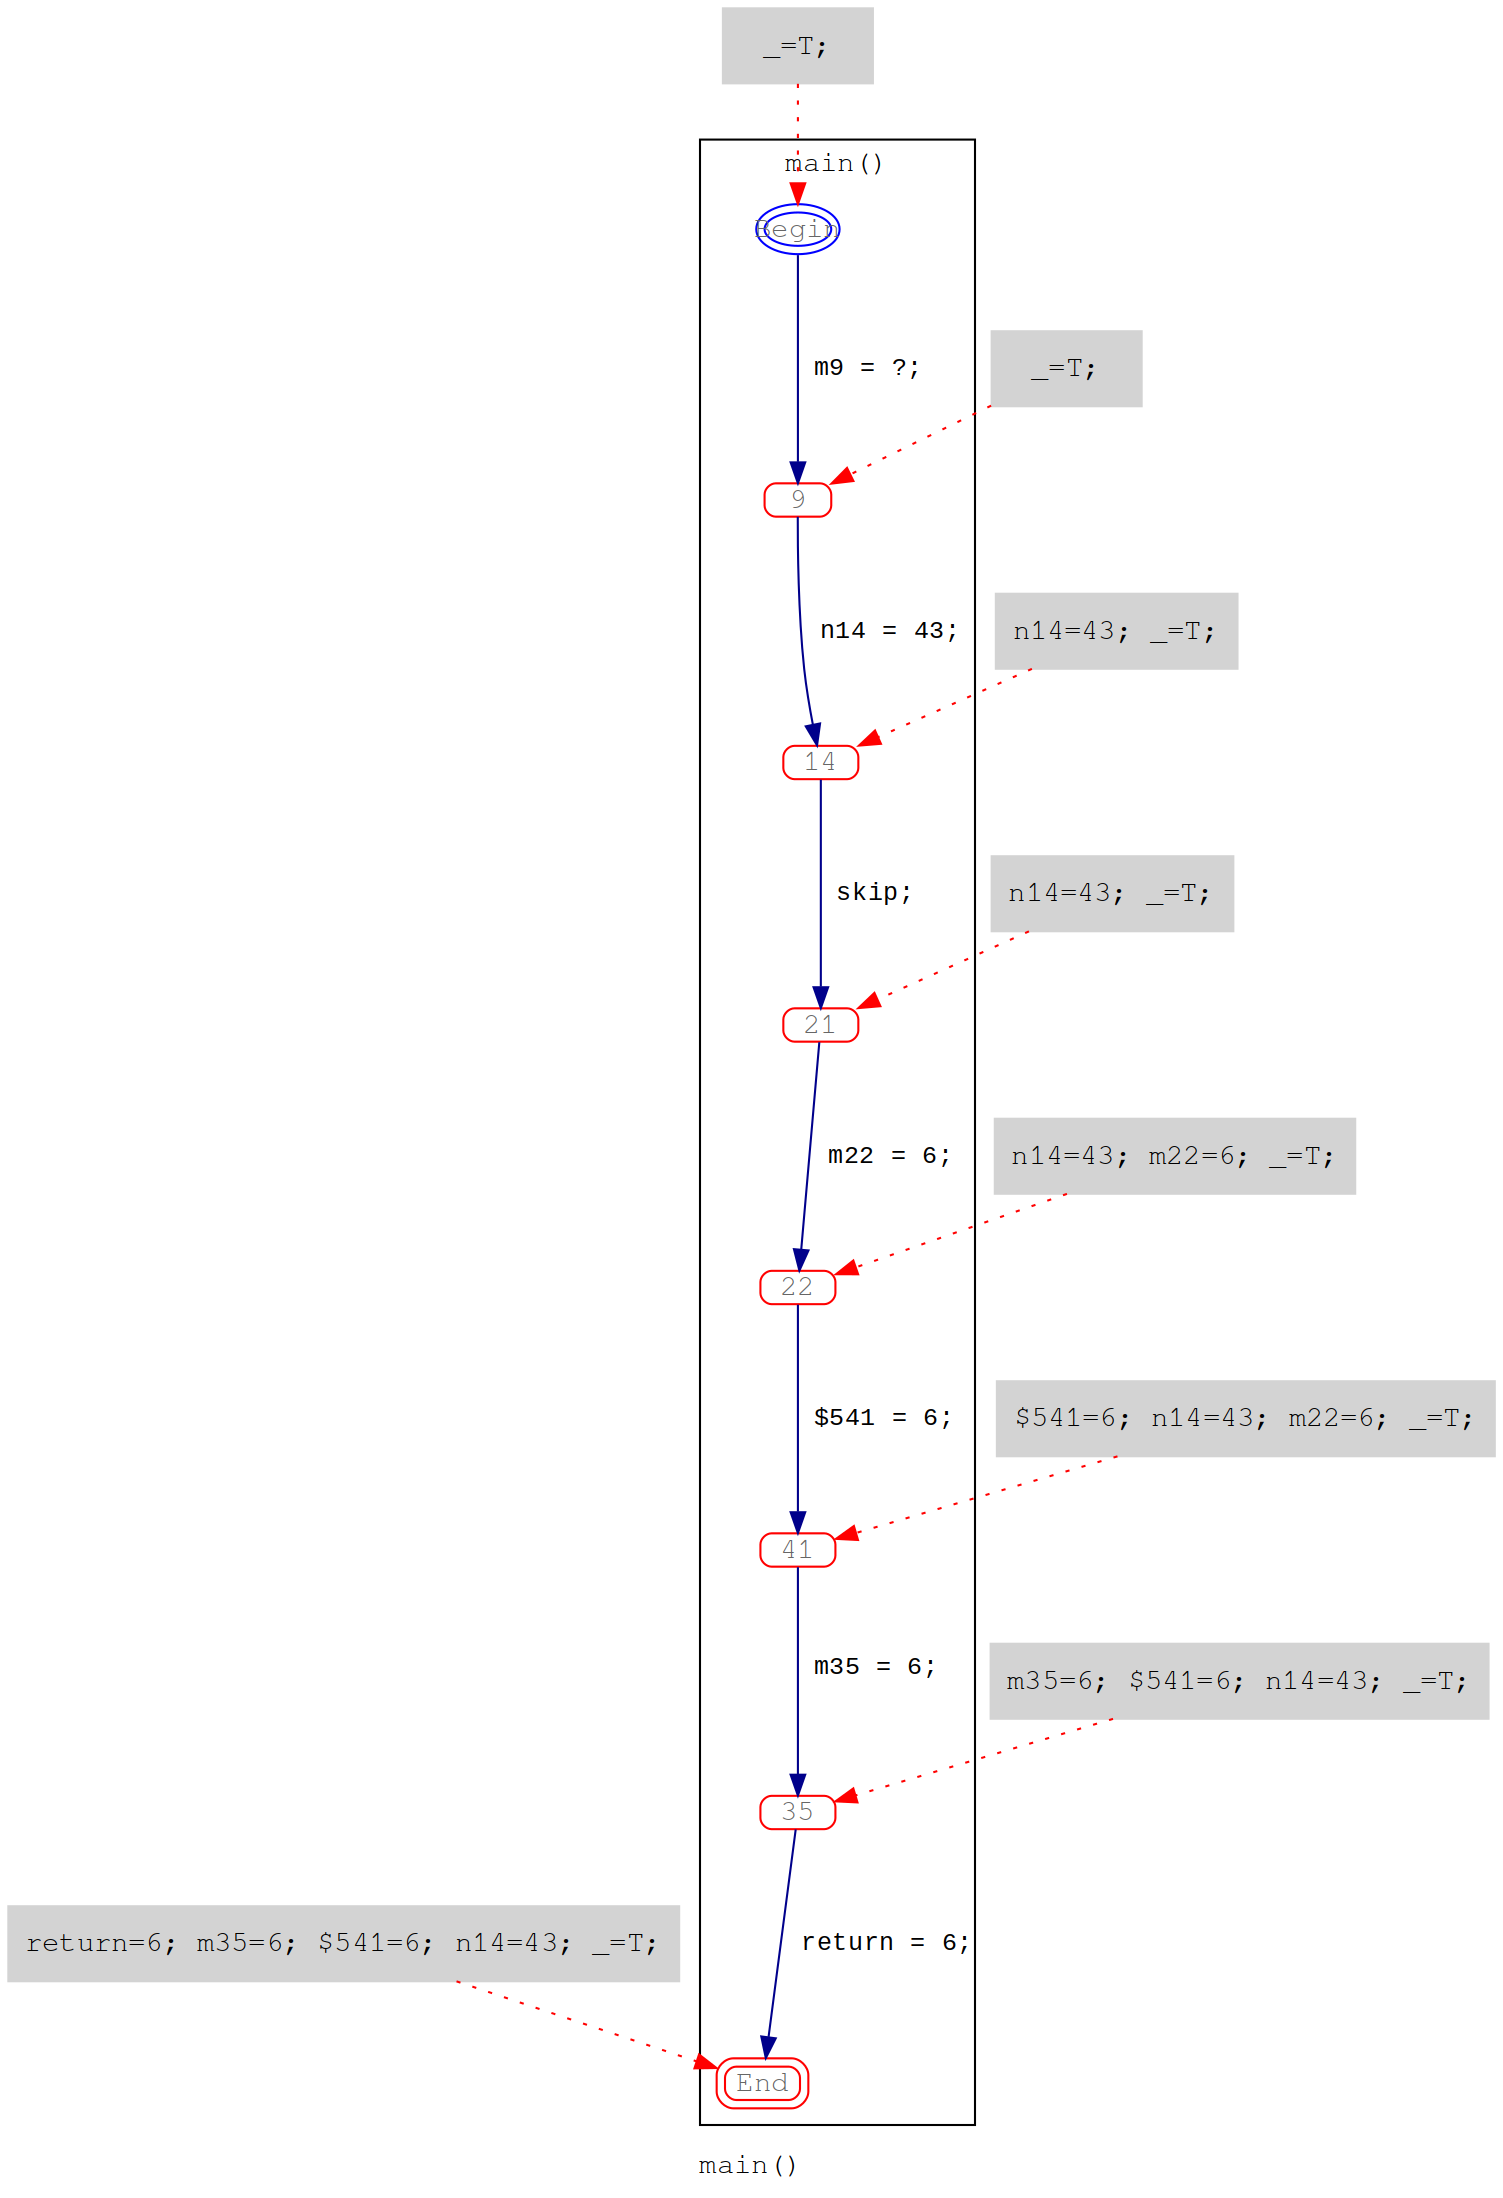
\includegraphics[height=7cm]{images/constfolding/example3b.png}

	The analysis can deduce that the condition is always true (\texttt{n15>5} for \texttt{n15 = 43}).
	Therefore remove the dead branch!
\end{frame}

%%%%%%%%%%%%%%%%%%%%%%%%%%%%%%%%%%%%%%%%%%%%%%%%%%%%%%%%%%%%%%%%%%%%%%%%%%%%%%%%
\begin{tumplainframe}{Thanks!}
\begin{center}
	\Huge Questions?
\end{center}
\end{tumplainframe}

\end{document}
